\frame
{
	\frametitle{Formulation}

	\begin{itemize}
	\item<1-> {\bf Input:} fully connected directed acyclic graph $G=(V,E)$ with source $s$ and sink $t$,
		and flow vector $f$.
	\end{itemize}

	\vspace{0.8cm}
	\begin{center}

\begin{tikzpicture}[font=\small,overlay,
mycirclex/.style={draw, circle, minimum size=1.0em, inner sep = 0.2mm}, 
mydiamond/.style={draw, diamond, minimum size=0.78em, inner sep = 0mm}, 
myrectang/.style={draw, rectangle, minimum size=0.60em, inner sep = 0mm}, 
>=stealth]

\def\cola{blue} 
\def\colb{orange}
\def\colc{mygreen}
\def\cold{purple} 
\def\cole{gray} 
\def\colf{cyan}
\def\colg{brown}


\def\len{1.3cm}

% G1
\begin{scope}[local bounding box=bbox, xshift=-6.6cm]
\path<3-> node[mycirclex] (vs) at (1.0 * \len, 0) {$s$};
\path<3-> node[mycirclex] (v1) at (2.0 * \len, 0) {$1$};
\path<3-> node[mycirclex] (v2) at (3.0 * \len, 0) {$2$};
\path<3-> node[mycirclex] (v3) at (4.0 * \len, 0) {$3$};
\path<3-> node[mycirclex] (v4) at (5.0 * \len, 0) {$4$};
\path<3-> node[mycirclex] (v5) at (6.0 * \len, 0) {$5$};
\path<3-> node[mycirclex] (v6) at (7.0 * \len, 0) {$6$};
\path<3-> node[mycirclex] (v7) at (8.0 * \len, 0) {$7$};
\path<3-> node[mycirclex] (vt) at (9.0 * \len, 0) {$t$};

\path<3-> [draw, \colx, ->, line width=0.04cm] (vs) -- (v1);
\path<3-> [draw, \colx, ->, line width=0.04cm] (v1) -- (v2);
\path<3-> [draw, \colx, ->, line width=0.04cm] (v2) -- (v3);
\path<3-> [draw, \colx, ->, line width=0.04cm] (v3) -- (v4);
\path<3-> [draw, \colx, ->, line width=0.04cm] (v4) -- (v5);
\path<3-> [draw, \colx, ->, line width=0.04cm] (v5) -- (v6);
\path<3-> [draw, \colx, ->, line width=0.04cm] (v7) -- (vt);

\path<3-> [draw, \colx, ->, line width=0.04cm, bend left = 50] (v1) to (v3);
\path<3-> [draw, \colx, ->, line width=0.04cm, bend left = 50] (v5) to (v7);
\path<3-> [draw, \colx, ->, line width=0.04cm, bend left = 50] (v6) to (vt);

\path<3-> node at (2 * \len, -0.36cm) {$5$};
\path<3-> node at (3 * \len, -0.36cm) {$1$};
\path<3-> node at (4 * \len, -0.36cm) {$5$};
\path<3-> node at (5 * \len, -0.36cm) {$5$};
\path<3-> node at (6 * \len, -0.36cm) {$5$};
\path<3-> node at (7 * \len, -0.36cm) {$3$};
\path<3-> node at (8 * \len, -0.36cm) {$2$};

\path<3-> node at (1.5 * \len, 0.2cm) {$5$};
\path<3-> node at (2.5 * \len, 0.2cm) {$1$};
\path<3-> node at (3.5 * \len, 0.2cm) {$1$};
\path<3-> node at (4.5 * \len, 0.2cm) {$5$};
\path<3-> node at (5.5 * \len, 0.2cm) {$5$};
\path<3-> node at (6.5 * \len, 0.2cm) {$3$};
\path<3-> node at (8.5 * \len, 0.2cm) {$2$};


\path<3-> node at (3.0 * \len, 0.9cm) {$4$};
\path<3-> node at (7.0 * \len, 0.9cm) {$2$};
\path<3-> node at (8.0 * \len, 0.9cm) {$3$};

\end{scope}
%\path<3-> [draw, rounded corners] ($(bbox.south west) - (0.00cm, 0.25cm)$) rectangle ($(bbox.north east) + (0.1cm, 0)$);
%\node at ($(bbox.south) - (0.00cm, 0.2cm)$) [label=below:{$G_2 - G_1 = \{c\}$}]{};


\end{tikzpicture}
\end{center}

	\vspace{-0.1cm}

	\begin{displaymath}
	M = \bordermatrix{
		~   & e_1 & e_2 & e_3 & e_4 & e_5 & e_6 & e_7 \cr
		p_1 & 1 & 1 & 1 & 1 & 0 & 0 & 0 \cr
		p_2 & 1 & 1 & 0 & 0 & 0 & 0 & 1 \cr
		p_3 & 1 & 0 & 0 & 1 & 0 & 1 & 0 \cr
		p_4 & 0 & 0 & 1 & 1 & 1 & 0 & 0 \cr
		p_5 & 0 & 0 & 0 & 0 & 1 & 0 & 1 \cr
	}
	\end{displaymath}

	\vspace{0.1cm}

	\begin{itemize}
	\item<1-> {\bf Output:} $P\subset R(M)$ {\bf and} vector $s$
		such that $f = s\cdot P$ and that $|R(P)|$ is minimized.
	\end{itemize}
}

\frame
{
	\frametitle{Facts}
	Let $\Delta = |E| - |V| + 2$. Let $(P^*, s^*)$ be any optimal solution.
	\vspace{0.3cm}
	\begin{itemize}
	\item<1-> {\bf Fact~1:} $rank(M) = \Delta$.
	\vspace{0.3cm}
	\item<1-> {\bf Fact~2:} $rank(P^*) = |R(P^*)|$.
	\vspace{0.3cm}
	\item<1-> {\bf Fact~3:} $|R(P^*)| \le \Delta$.
	\vspace{0.3cm}
	\item<1-> {\bf Fact~4:} If $|R(M)| = \Delta$, then the solution is unique: $(M, s)$, where
		$s$ is determined by $f = s\cdot M$. ({\it trivial cases})
	\vspace{0.3cm}
	\item<1-> {\bf Fact~5:} If $|R(P^*)| = \Delta$, then greedy algorithm is guarenteed to give optimal solution. ({\it easy cases})
	\vspace{0.3cm}
	\item<1-> {\bf Degenerated cases:} $|R(P^*)| < \Delta$. ({\it hard cases})
	\end{itemize}
}

\frame
{
	\frametitle{Degeneration Theorem}
	%\begin{itemize}
	%\item Degenerated example~($rank(P^*) = 3$, $\Delta = 4$).
	%\end{itemize}

	\vspace{0.4cm}
	\begin{center}

\begin{tikzpicture}[font=\small,overlay,
mycirclex/.style={draw, circle, minimum size=1.0em, inner sep = 0.2mm}, 
mydiamond/.style={draw, diamond, minimum size=0.78em, inner sep = 0mm}, 
myrectang/.style={draw, rectangle, minimum size=0.60em, inner sep = 0mm}, 
>=stealth]

\def\cola{blue} 
\def\colb{orange}
\def\colc{mygreen}
\def\cold{purple} 
\def\cole{gray} 
\def\colf{cyan}
\def\colg{brown}


\def\len{1.8cm}

% G1
\begin{scope}[local bounding box=bbox, xshift=-6.4cm]
\path<1-> node[mycirclex] (v1) at (1.0 * \len, 0) {$s$};
\path<1-> node[mycirclex] (v2) at (2.0 * \len, 0) {$a$};
\path<1-> node[mycirclex] (v3) at (3.0 * \len, 0) {$b$};
\path<1-> node[mycirclex] (v4) at (4.0 * \len, 0) {$c$};
\path<1-> node[mycirclex] (v5) at (5.0 * \len, 0) {$d$};
\path<1-> node[mycirclex] (v6) at (6.0 * \len, 0) {$t$};

\path<1-> [draw, \colx, ->, line width=0.04cm] (v1) -- (v2);
\path<1-> [draw, \colx, ->, line width=0.04cm] (v2) -- (v3);
\path<1-> [draw, \colx, ->, line width=0.04cm] (v3) -- (v4);
\path<1-> [draw, \colx, ->, line width=0.04cm] (v4) -- (v5);
\path<1-> [draw, \colx, ->, line width=0.04cm] (v5) -- (v6);

\path<1-> [draw, \colx, ->, line width=0.04cm, bend left = 40] (v1) to (v3);
\path<1-> [draw, \colx, ->, line width=0.04cm, bend left = 40] (v3) to (v5);
\path<1-> [draw, \colx, ->, line width=0.04cm, bend left =-40] (v2) to (v5);
\path<1-> [draw, \colx, ->, line width=0.04cm, bend left =-40] (v4) to (v6);

\path<1-> node at (1.5 * \len, 0.2cm) {$4$};
\path<1-> node at (2.5 * \len, 0.2cm) {$1$};
\path<1-> node at (3.5 * \len, 0.2cm) {$5$};
\path<1-> node at (4.5 * \len, 0.2cm) {$4$};
\path<1-> node at (5.5 * \len, 0.2cm) {$9$};

\path<1-> node at (2.0 * \len, 1.0cm) {$6$};
\path<1-> node at (4.0 * \len, 1.0cm) {$2$};
\path<1-> node at (5.0 * \len,-1.0cm) {$1$};
\path<1-> node at (3.5 * \len,-1.3cm) {$3$};

\end{scope}
%\path<1-> [draw, rounded corners] ($(bbox.south west) - (0.00cm, 0.25cm)$) rectangle ($(bbox.north east) + (0.1cm, 0)$);
%\node at ($(bbox.south) - (0.00cm, 0.2cm)$) [label=below:{$G_2 - G_1 = \{c\}$}]{};


\end{tikzpicture}
\end{center}


	\vspace{-0.4cm}

	\begin{displaymath}
	\bordermatrix{
		~   & e_1 & e_2 & e_3 & e_4 & e_5 & e_6\cr
		p_1 & 1 & 0 & 1 & 0 & 0 & 1 \cr
		p_2 & 1 & 0 & 0 & 1 & 1 & 0 \cr
		p_3 & 0 & 1 & 1 & 0 & 1 & 0 \cr
	} 
	\bordermatrix{
   	   ~& q_1 & q_2 & q_3 \cr
		& +1 &  0 & +1  \cr
		& +1 &  0 &  0  \cr
		& -1 & +1 &  0  \cr
		& -1 & +1 & -1  \cr
		&  0 & -1 &  0  \cr
		&  0 & -1 & -1  \cr
	} = 0
	\end{displaymath}

	\begin{itemize}
	\item Consider the {\bf null space} of $P^*$, i.e., $N(P^*) = \{q | P^*\cdot q = 0\}$.
	\item $\dim(N(P^*)) = |E| - rank(P^*) = |E| - |R(P^*)|$. 
	\item For any $q\in N(P)$, we have $f\cdot q = s\cdot P \cdot q = 0$. 
	\item {\bf Theorem:} There exists $\Delta - |R(P^*)|$ linearly independent non-trivial vectors
	satisfying $f\cdot q = 0$.
	\end{itemize}
}

\frame
{
	\frametitle{Identifying Equations}
	\begin{itemize}
	\item {\bf Conjecture:} $q_i \in \{+1, -1, 0\}$.
	\vspace{0.2cm}
	\item Only consider two simple orms of equations in the current implementation:
		\begin{align}
		f_i & =  f_{i_1} + f_{i_2} + \cdots + f_{i_k} \tag{a}\\
		f_i + f_j & = f_{i_1} + f_{i_2} + \cdots + f_{i_k} \tag{b}
		\end{align}
	\item {\bf Algorithm:} Use the existing pseudo-polynomial-time algorithm for the subset-sum problem.
	\vspace{0.2cm}
	\item For equation of form (a): split $e_i$ into $k$ edges, each with flow
	value of $f_{i_k}$; record these $k$ pairs of edges with equal flow.
	\vspace{0.2cm}
	\item For equation of form (b): use heuristics to split both sides into
			identical set of edges; record these pairs with equal flow.
	\end{itemize}
}

\frame
{
	\frametitle{Merge Adjacent Edges with Equal Flow}
	\vspace{-2.0cm}

	\begin{itemize}
	\item {\bf Algorithm:} merge them directly.
	\end{itemize}

	\vspace{0.8cm}
	\input{figs/graph3.tex}

}


\frame
{
	\frametitle{Merge Distant Edges with Equal Flow}
	\vspace{-3.0cm}

	\begin{itemize}
	\item {\bf Algorithm:} swap and exchange subgraphs based on the its (partial) {\bf nested} structure.
	\end{itemize}

	\vspace{0.8cm}
	\input{figs/graph4.tex}

}

\frame
{
	\frametitle{Algorithm}
	\begin{itemize}
	\item Iterate until no change is made to the graph
		\vspace{0.2cm}
		\begin{itemize}
		\item[1.] Decompose trivial vertices
		\vspace{0.2cm}
		\item[2.] Identify type~(a) equation and split it
		\vspace{0.2cm}
		\item[3.] Merge equal edges that can be made adjacent
		\vspace{0.2cm}
		\item[4.] Merge equal edges that can not be made adjacent~(*)
		\vspace{0.2cm}
		\item[5.] Identify type~(b) equation and split it~(*)
		\vspace{0.2cm}
		\end{itemize}
	\item Arbitrarily decompose the remaining graph using greedy algorithm
	\end{itemize}
}

\frame
{
	\frametitle{Simulation Results}

	\begin{itemize}
	\item Use iGenome annotation~(gtf file) of Human genome.
	\vspace{0.2cm}
	\item Use Flux Simulator to only simulate expression levels~(all with default parameters).
	\vspace{0.2cm}
	\item Simulate independently 100 instances and compute their average.
	\vspace{0.2cm}
	\end{itemize}

	\def\SA{\hspace*{0pt}}
	\def\SC{\hspace*{-2pt}}
	\def\SB{\hspace*{1pt}}
	\def\SD{\hspace*{3pt}}

	\begin{center}%
		\setlength{\tabcolsep}{0.9pt}%
		\begin{tabular}{cccccccccccccccccccccccccccc}%
		\hline
		     & #genes & #trivial & #easy & #hard & greedy & scallop &
		mean & 11376.5 & 8212.9 & 128.8 & 3034.9& 98.4 & 7.5 &
		std  & 86.7 & 51.6 & 4.9 & 39.6 & 4.2 & 2.8 &
		\hline\noalign{\smallskip}%
		\end{tabular}%
	\end{center}%
}
